\begin{figure}[H]
    \centering
    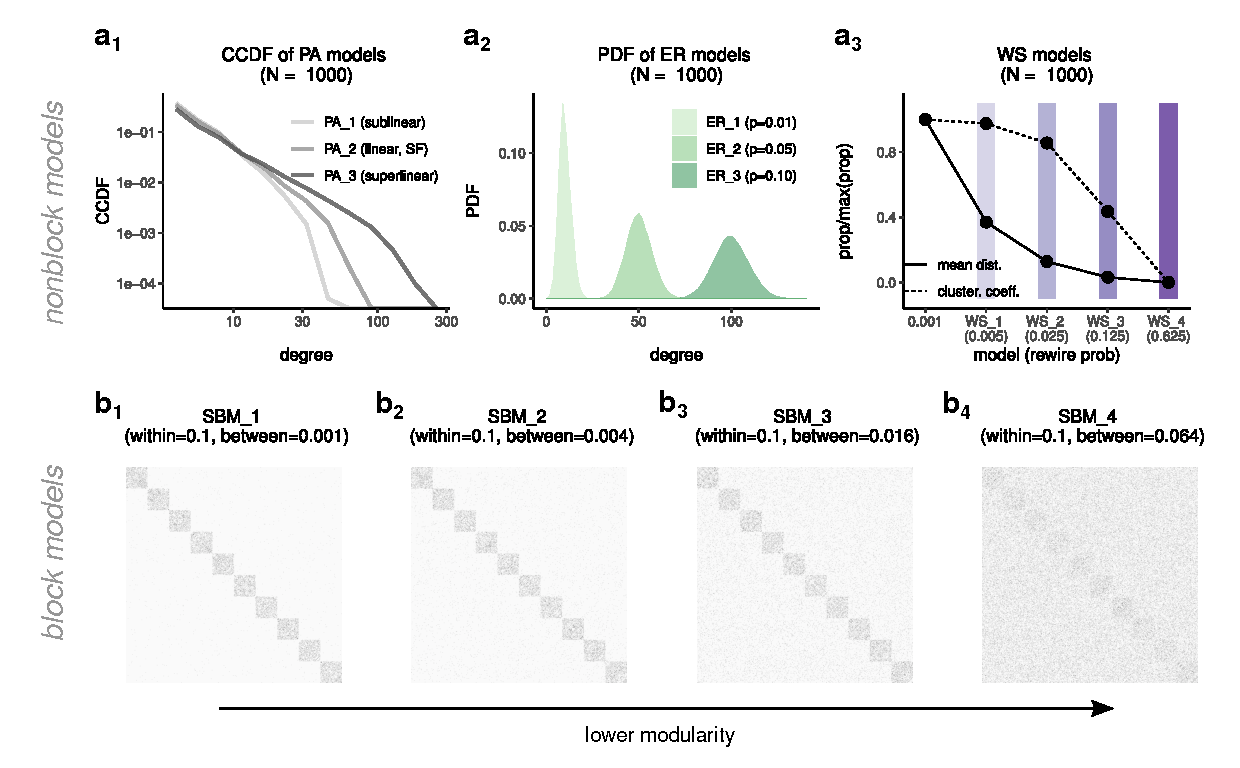
\includegraphics[width=0.95\textwidth,center]{../figures/report/Fig2.pdf}
    \caption{\label{fig:2}
    \textit{Examples of intralayer static model set up}. For simplicity, for all instances, the types of models used are the same for both agent and topic graph.
    (\textbf{a}) Non-block models (PA: preferential attachment, ER: Erdős–Rényi, WS: Watts–Strogatz; see method for more details). (\textbf{b}) Stochastic block models (SBM) with decreasing modularity by increasing the connection probability between members of different groups. There are 10 groups for each intralayer model.
    }
\end{figure}